\documentclass{article}
\usepackage{arxiv}

\usepackage[utf8]{inputenc} % allow utf-8 input
\usepackage[T1]{fontenc}    % use 8-bit T1 fonts
\usepackage{hyperref}       % hyperlinks
\usepackage{url}            % simple URL typesetting
\usepackage{booktabs}       % professional-quality tables
\usepackage{amsfonts}       % blackboard math symbols
\usepackage{nicefrac}       % compact symbols for 1/2, etc.
\usepackage{microtype}      % microtypography
\usepackage{cleveref}       % smart cross-referencing
\usepackage{lipsum}         % Can be removed after putting your text content
\usepackage{graphicx}
\usepackage[numbers]{natbib}
\usepackage{doi}

\title{Project Proposal: Counting card system for Blackjack}

% Here you can change the date presented in the paper title
%\date{September 9, 1985}
% Or remove it
\date{}

\newif\ifuniqueAffiliation
% Comment to use multiple affiliations variant of author block 
\uniqueAffiliationtrue

\ifuniqueAffiliation % Standard variant of author block
\author{{\hspace{1mm}Davide Baggio 2122547} \\
	Department of Computer Engineering\\
	University of Padua\\
	%% examples of more authors
	\And
	{\hspace{1mm}Zoren Martinez 2123873} \\
	Department of Computer Engineering\\
	University of Padua\\
	\And
	{\hspace{1mm}Francesco Pivotto 2158296} \\
	Department of Computer Engineering\\
	University of Padua\\
}
\else
% Multiple affiliations variant of author block
\usepackage{authblk}
\renewcommand\Authfont{\bfseries}
\setlength{\affilsep}{0em}
% box is needed for correct spacing with authblk
\newbox{\orcid}\sbox{\orcid}{\includegraphics[scale=0.06]{orcid.pdf}} 
\author[1]{%
	{\usebox{\orcid}\hspace{1mm}Davide Baggio}
}
\author[1,2]{%
	{\usebox{\orcid}\hspace{1mm}Zoren Martinez}
}
\affil[1]{Department of Computer Engineering, University of Padua}
\affil[2]{Department of Computer Engineering, University of Padua}
\fi

% Uncomment to override  the `A preprint' in the header
\renewcommand{\headeright}{}
\renewcommand{\undertitle}{}
\renewcommand{\shorttitle}{Project Proposal: Counting card system for Blackjack}

%%% Add PDF metadata to help others organize their library
%%% Once the PDF is generated, you can check the metadata with
%%% $ pdfinfo template.pdf
\hypersetup{
pdftitle={Project Proposal: Counting card system for Blackjack},
pdfauthor={Davide Baggio, Zoren Martinez, Francesco Pivotto},
}

\begin{document}
\maketitle


% how to cite: \cite{stefano2021}
% ref a figure \ref{fig:fig1}

% display figure
%\begin{figure}
%	\centering
%	\fbox{\rule[-.5cm]{4cm}{4cm} \rule[-.5cm]{4cm}{0cm}}
%	\caption{Sample figure caption.}
%	\label{fig:fig1}
%\end{figure}

% display table
% \begin{table}
% 	\caption{Sample table title}
% 	\centering
% 	\begin{tabular}{lll}
% 		\toprule
% 		\multicolumn{2}{c}{Part}                   \\
% 		\cmidrule(r){1-2}
% 		Name     & Description     & Size ($\mu$m) \\
% 		\midrule
% 		Dendrite & Input terminal  & $\sim$100     \\
% 		Axon     & Output terminal & $\sim$10      \\
% 		Soma     & Cell body       & up to $10^6$  \\
% 		\bottomrule
% 	\end{tabular}
% 	\label{tab:table}
% \end{table}

\section*{Introduction}

In the realm of casino gaming, ensuring fair play and detecting potential cheating behaviors is of paramount importance. One such method of cheating that has persisted over time is card counting in the game of Blackjack. While not inherently illegal, card counting can give players a significant advantage over the house, leading to potential revenue losses for casinos. As a response to this challenge, this project proposes the development of an automated card counting detection system using C++, OpenCV, and potentially deep learning techniques.

The core objective of the project is to build a real-time video analysis system capable of observing and interpreting the flow of cards dealt in Blackjack games. By leveraging the capabilities of OpenCV for image processing and card recognition, combined with the power of C++ for performance and control, the system will track the sequence of cards on the table. Additionally, machine learning or deep learning algorithms may be integrated to analyze patterns in player behavior and betting in correlation with card distributions, flagging potential instances of card counting.

This automated system has practical implications for modern casinos, offering an intelligent and scalable solution to monitor gameplay, support security teams, and uphold the integrity of the game without intrusive surveillance. Through this project, we aim to contribute to the development of smart surveillance tools in gaming environments using cutting-edge computer vision and AI technologies.

\section*{Visual Output and Card Value Representation}

To facilitate intuitive monitoring and real-time analysis, the system will process the video feed and overlay bounding boxes around detected playing cards. Each bounding box will be color-coded based on the card's value in the Hi-Lo counting system:

\begin{itemize}
	\item \textbf{Green} bounding boxes will indicate cards valued at +1 (typically 2 through 6).
	\item \textbf{Blue} bounding boxes will indicate neutral cards with a value of 0 (typically 7 through 9).
	\item \textbf{Red} bounding boxes will indicate high-value cards that subtract from the count, assigned a value of -1 (typically 10, face cards, and Aces).
\end{itemize}

This visual overlay will not only aid in debugging and performance evaluation but will also allow casino personnel to interpret the system's counting logic in real time. By observing the count trend and the corresponding card values, operators can better assess whether a player’s betting behavior aligns suspiciously with card distribution—potentially identifying card counting activity.

This color-coded visualization enhances transparency and provides immediate visual cues without requiring technical expertise to understand the underlying card tracking mechanism.

\begin{figure}[htbp]
    \centering
    \begin{minipage}{0.45\textwidth}
        \centering
        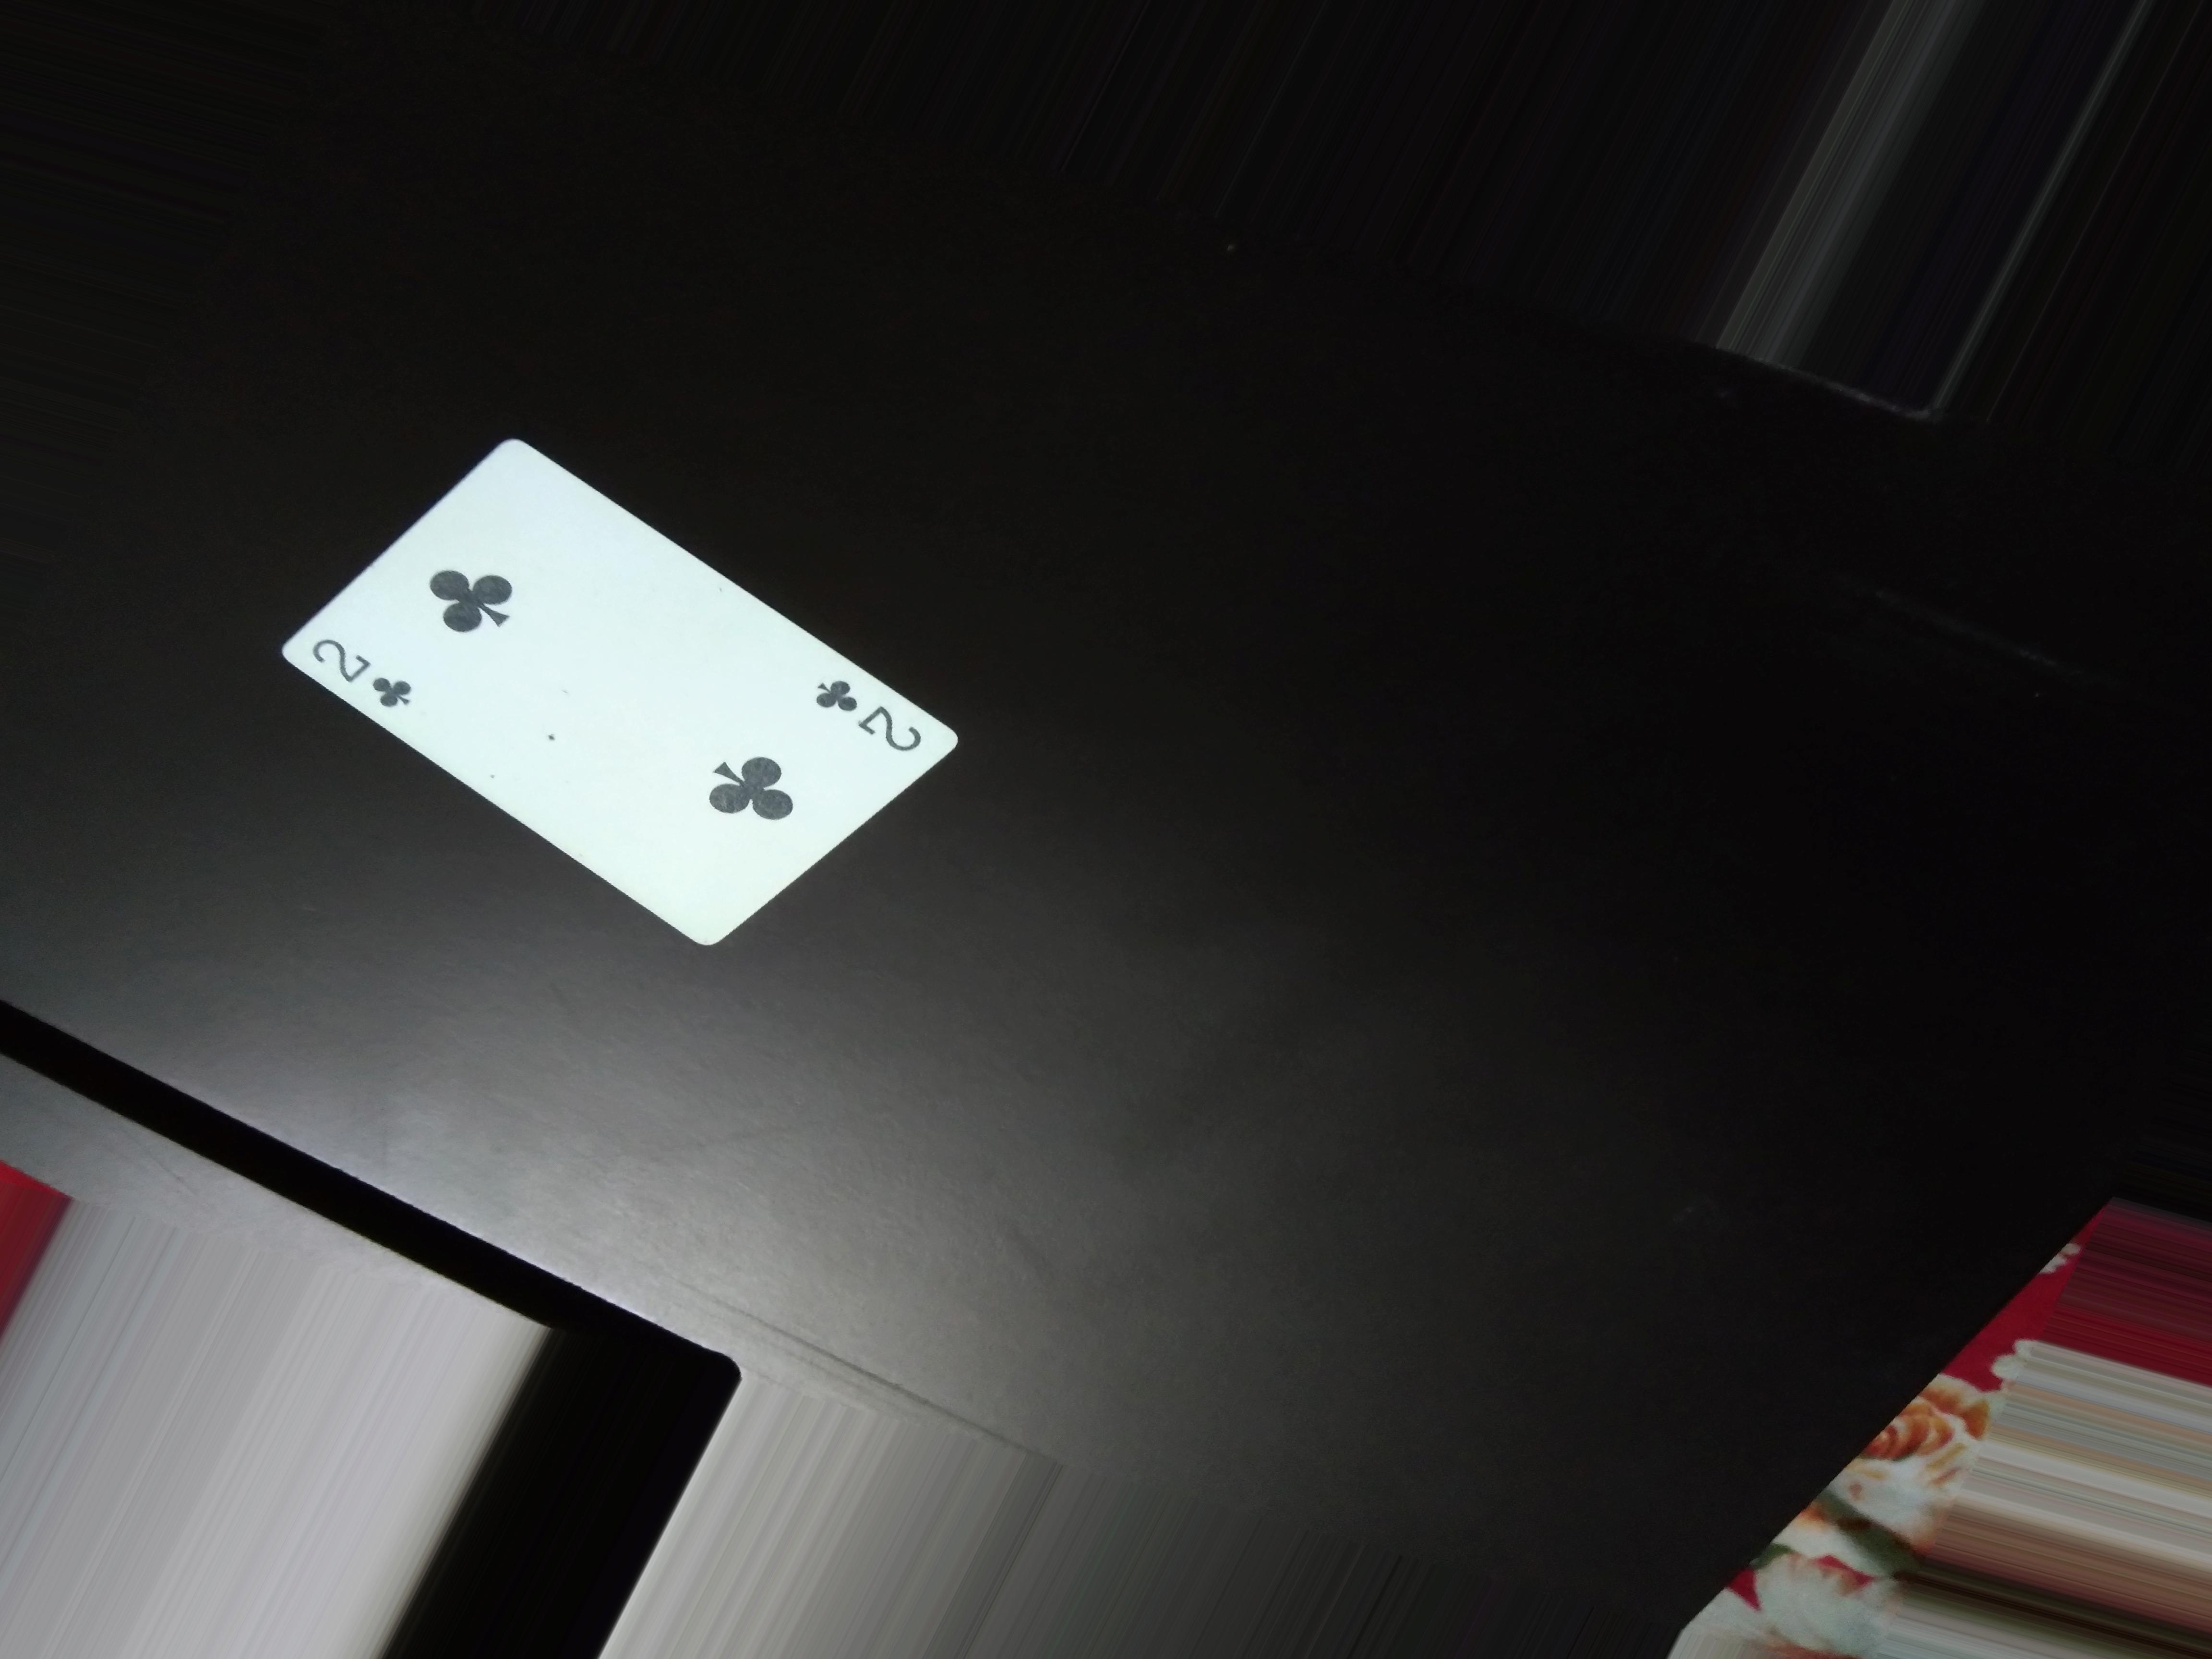
\includegraphics[width=\linewidth]{./assets/2C40.jpg}
    \end{minipage}
    \hfill
    \begin{minipage}{0.45\textwidth}
        \centering
        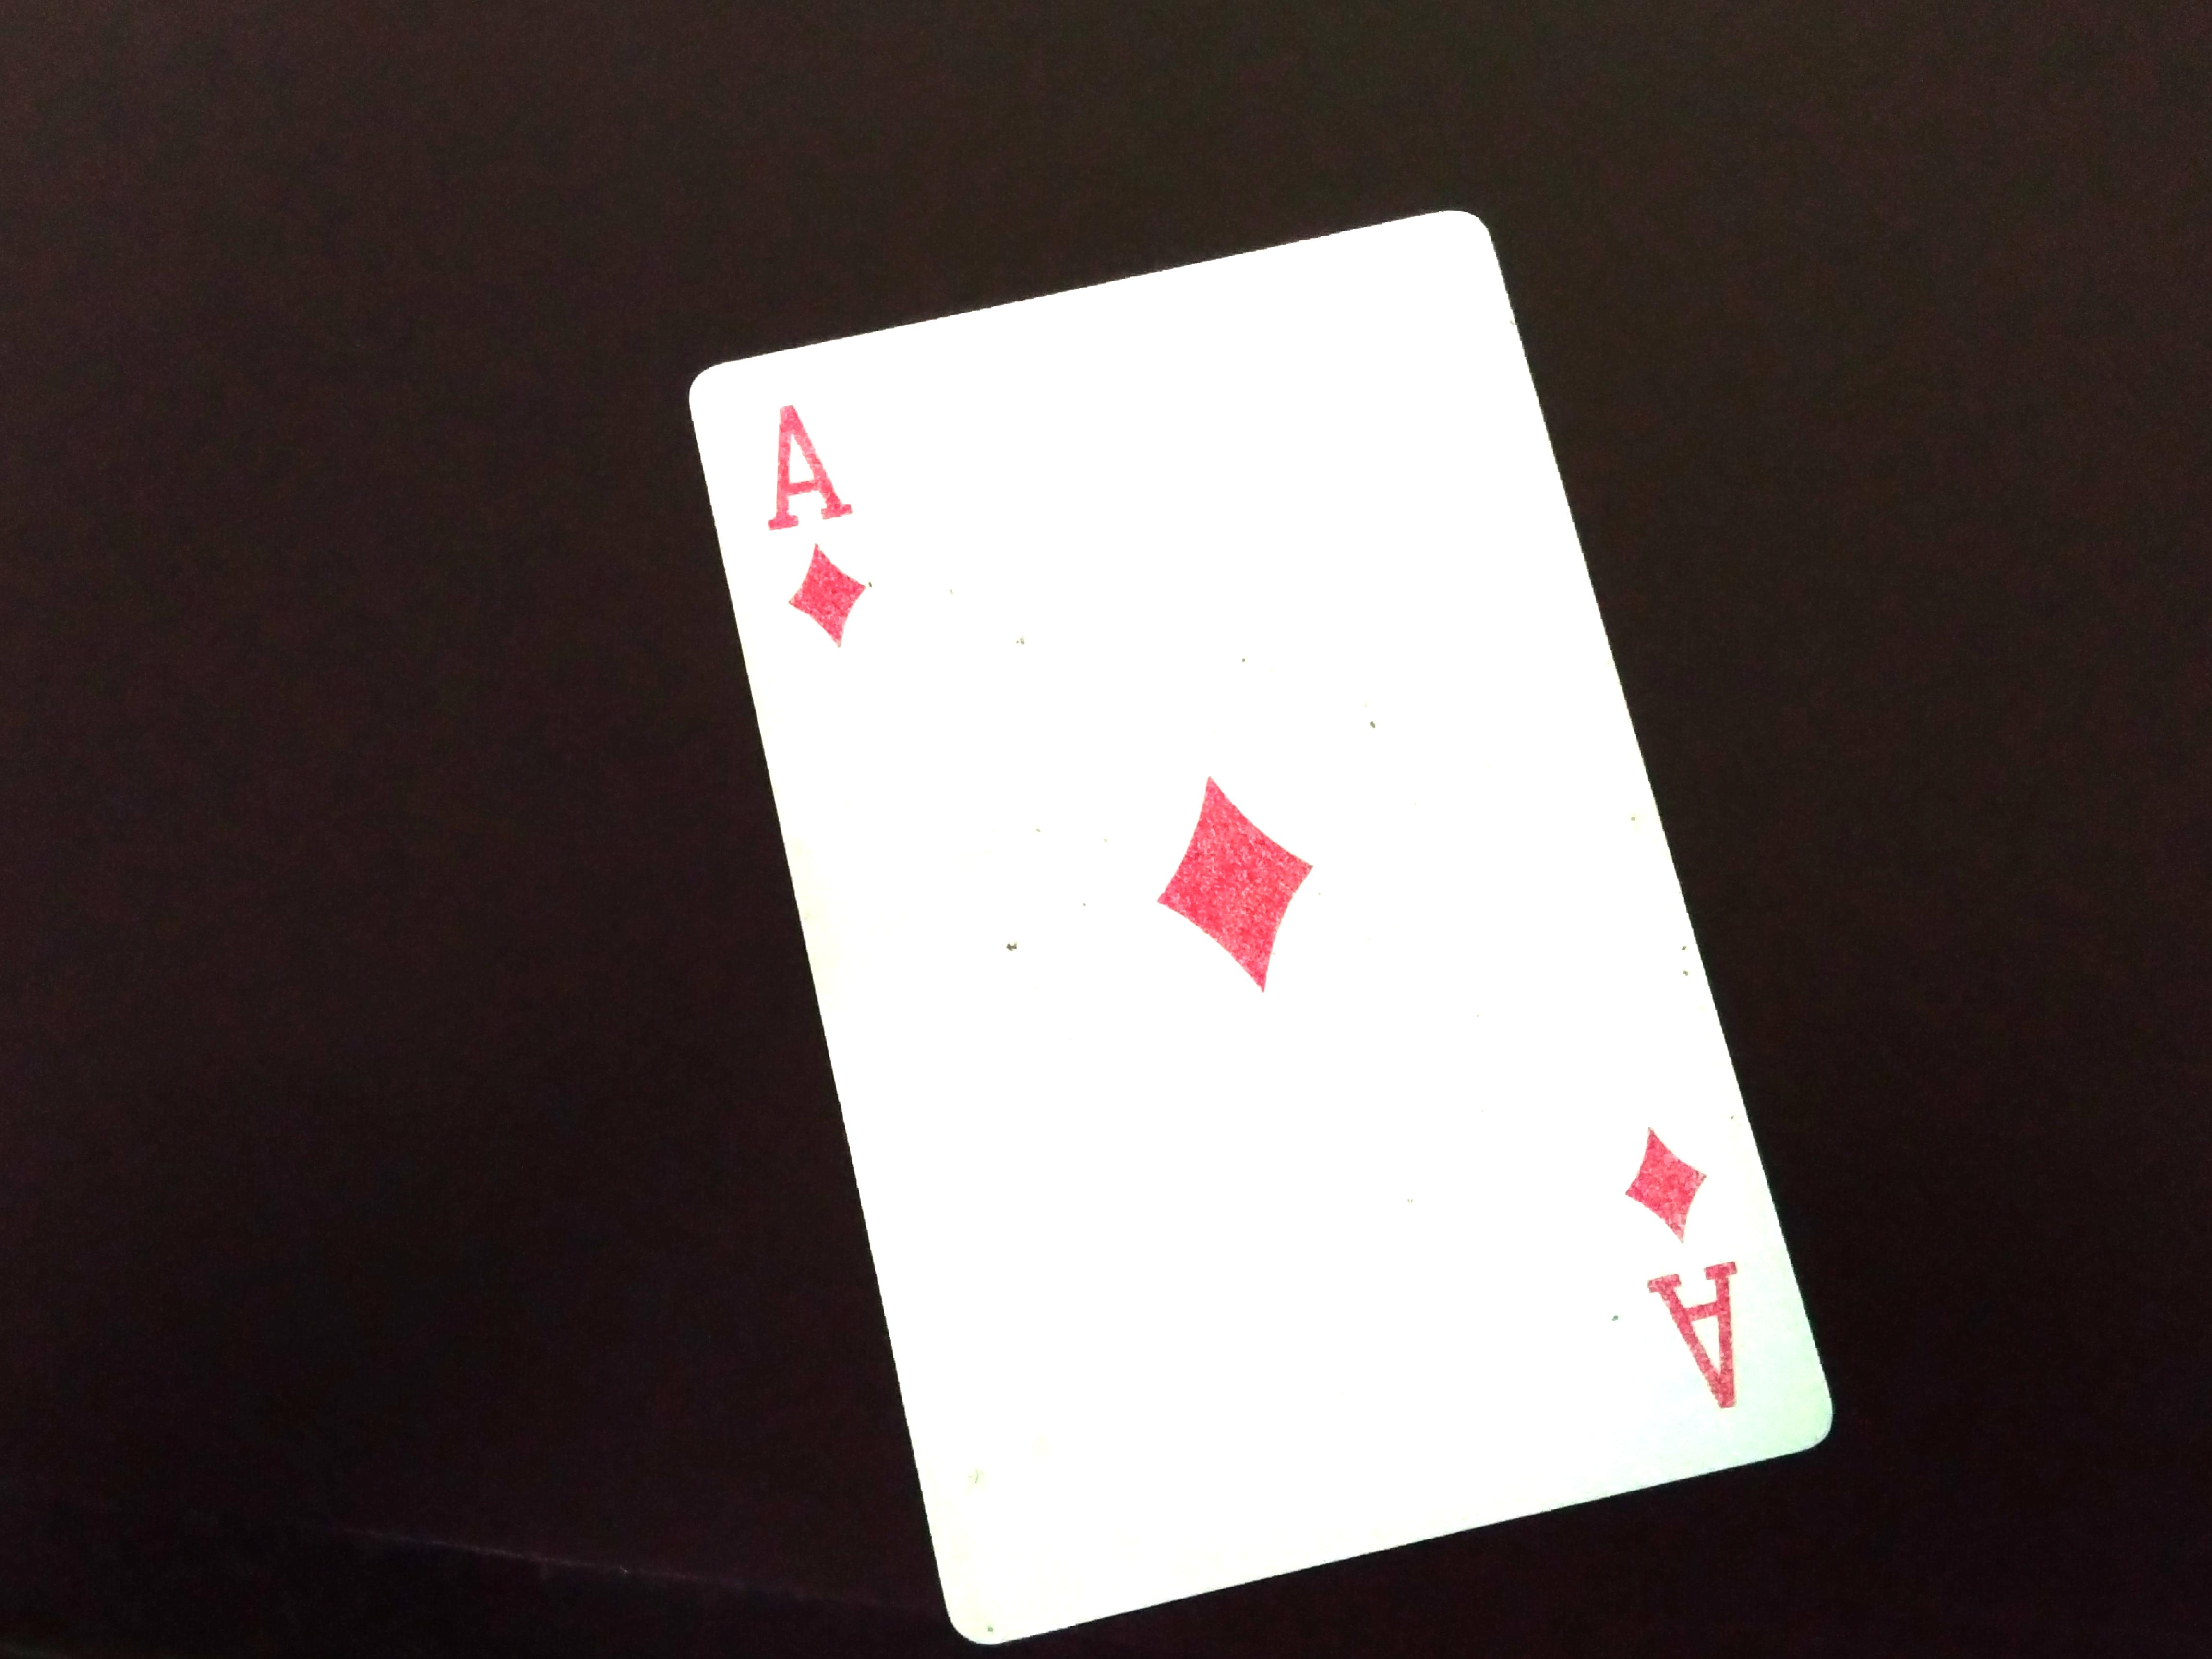
\includegraphics[width=\linewidth]{./assets/AD48.jpg}
    \end{minipage}
	\caption{Sample images}
    \label{fig:fig1}
\end{figure}

\begin{figure}[htbp]
    \centering
    \begin{minipage}{0.45\textwidth}
        \centering
        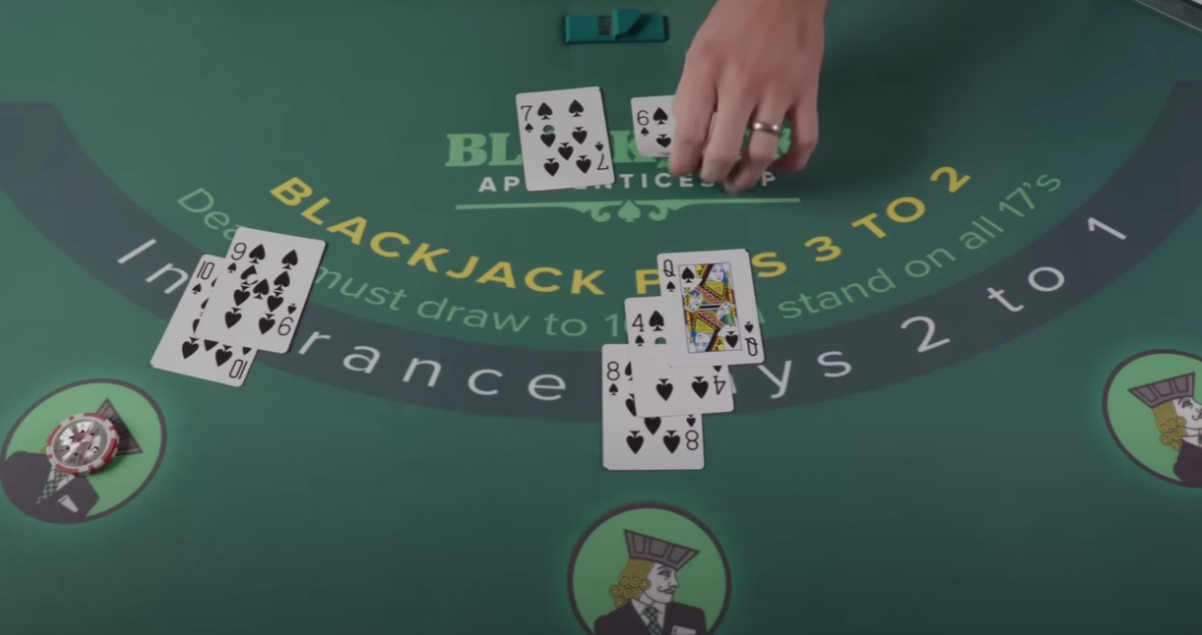
\includegraphics[width=\linewidth]{./assets/example_default.png}
        \caption{(a) Base image}
    \end{minipage}
    \hfill
    \begin{minipage}{0.45\textwidth}
        \centering
        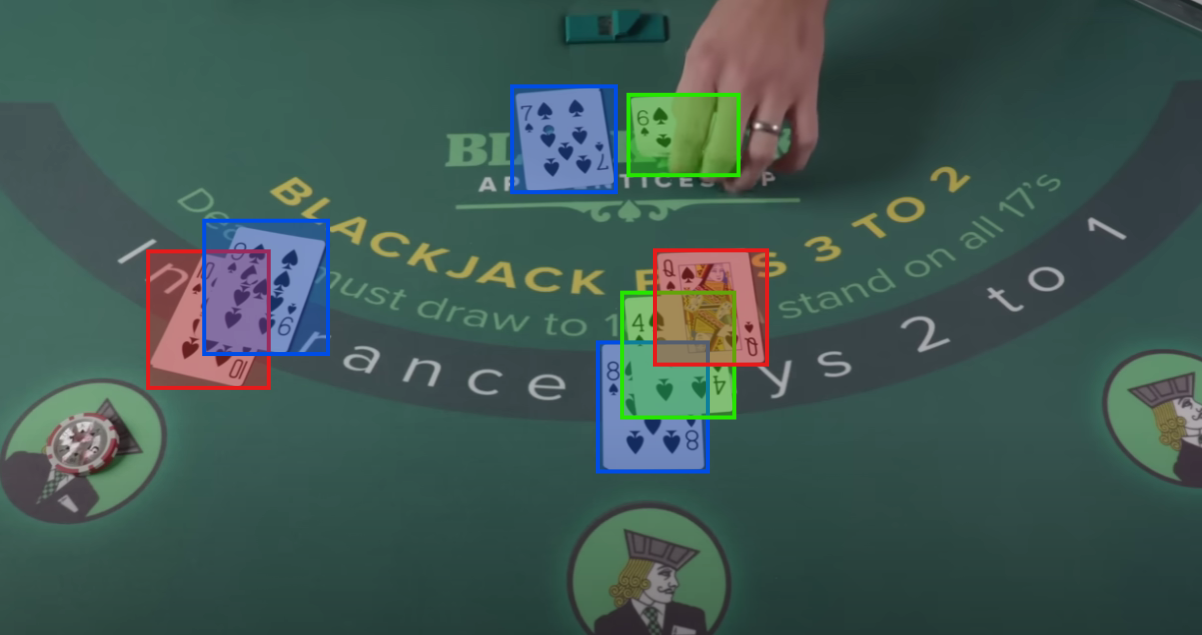
\includegraphics[width=\linewidth]{./assets/example_detected.png}
        \caption{(b) Detection output}
    \end{minipage}
    \label{fig:fig2}
\end{figure}

\section*{Dataset and Real-World Data Sources}

To train and evaluate the card detection and recognition system, we will utilize a combination of a structured dataset and real-world video footage:

\subsection*{The Complete Playing Card Dataset}

We will employ the Complete Playing Card Dataset \cite{jay2020} available on Kaggle. This dataset comprises approximately 50 images for each playing card, including Jokers. Each card serves as a distinct class, providing a diverse set of images that capture various positions and rotations of the cards. This diversity is crucial for training a robust model capable of recognizing cards under different orientations and perspectives.

\subsection*{Real-World Video Footage}

To simulate real-time scenarios and evaluate the system's performance in practical environments, we will use publicly available Blackjack gameplay videos sourced from platforms like YouTube. These videos offer a variety of real-world conditions, including different lighting, backgrounds, and card arrangements, which are essential for testing the system's robustness and adaptability.

By combining the structured dataset with real-world video footage, we aim to develop a comprehensive card counting detection system that performs reliably in both controlled and dynamic environments.

\section*{Performance Measurement}

To ensure the reliability and practicality of the proposed card counting detection system, a comprehensive evaluation strategy will be implemented. The performance of the system will be assessed across several key metrics, focusing on both the card recognition accuracy and the effectiveness of the card counting logic in real-world conditions.

\subsection*{Card Detection and Recognition Accuracy}

The first layer of performance measurement involves evaluating how accurately the system detects and classifies individual playing cards:

\begin{itemize}
	\item The mean Average Precision (mAP);
	\item The mean Intersection over Union (mIoU);
\end{itemize}

In case some machine learning models are developed we are going to use these metrics too: 

\begin{itemize}
	\item Precision and Recall: These will be measured to assess the system’s ability to correctly identify cards (true positives) while minimizing false detections.
	\item F1-Score: A harmonic mean of precision and recall to provide a balanced evaluation metric.
	\item Confusion Matrix: To visualize misclassifications across different card types and values.
\end{itemize}

Testing will be performed on:

\begin{itemize}
	\item Held-out images from the annotated dataset (to test generalization).
	\item Frames extracted from real gameplay videos, where ground truth labels are manually annotated for evaluation purposes.
\end{itemize}
\newpage
\section*{Post-Feedback Clarifications and Additions}

\subsection*{Handling Occlusions}

Occlusions can be a significant challenge, particularly due to players’ hands or overlapping cards. We plan to address these cases with two strategies:

\begin{itemize}
    \item \textbf{Short-term occlusions (e.g., by hands)} will be handled using temporal tracking techniques. The key idea is to retain memory of previous frames: if a card was clearly visible at a certain position before the occlusion, and something now covers that same area, we can reasonably assume (within a short time window) that the card is still there. Thus, we will maintain a short history buffer to preserve card positions through minor occlusions.
    
    \item \textbf{Occlusions between cards} are more complex. In such cases, we aim to estimate the full extent of a partially visible card by analyzing the visible portion (i.e., the suit and rank). Based on the size and position of these features, we will infer the probable dimensions and orientation of the complete card, projecting the likely full bounding box even if the card is partially covered by another.
\end{itemize}

\subsection*{Annotation Strategy}

Our evaluation pipeline involves two types of data sources:

\begin{itemize}
    \item A subset of the \textit{Complete Playing Card Dataset} from Kaggle, which contains isolated card images without blackjack context. This dataset already includes full annotations, which we will use to evaluate basic card detection accuracy in controlled conditions.
    
    \item Real-world gameplay videos sourced from YouTube. For this data, we will manually annotate selected frames with bounding boxes and corresponding Hi-Lo values. Due to the manual nature of this process, we will limit the number of annotated frames and avoid using excessively long video sequences.
\end{itemize}

Each bounding box will be labeled according to the Hi-Lo counting value of the card: $+1$, $0$, or $-1$.

\subsection*{Addition of Accuracy Metric}

As suggested, we will include \textbf{accuracy} among the evaluation metrics to better assess the relationship between true positives and the total number of detections. Accuracy will be calculated using the standard formula:

\[
\text{Accuracy} = \frac{TP + TN}{TP + TN + FP + FN}
\]

where $TP$ = True Positives, $TN$ = True Negatives, $FP$ = False Positives, and $FN$ = False Negatives.

\subsection*{Test Data Variability}

To assess robustness, we plan to test the system on gameplay videos with varying backgrounds (e.g., different table colors). However, we were not able to find suitable videos from multiple viewpoints. Despite this, we will strive to select videos with realistic variability in lighting and card layout conditions to simulate diverse gameplay environments as closely as possible.


%\subsection*{Accuracy of Card Counting Logic}
%
%The system’s ability to maintain an accurate running count will be verified by comparing its output with manually computed counts based on recorded game sessions. Metrics include:
%
%Running Count Error Rate: Average deviation of the system's count from the ground truth over time.
%
%Event-Based Accuracy: Correct detection of count transitions (e.g., from neutral to positive count, or negative to neutral).

\nocite{*}

\bibliographystyle{plainurl}
\bibliography{references}
\end{document}